% fig_datapath.tex - the whole single-cycle core (rtl/riscv_core.sv), with the
% five stage modules shaded. Wire names are the riscv_core signal names.
% Control selects are drawn as named dashed stubs at their destination; the
% control unit lists them. Rounded flags (e.g. [rs2_data]) are net labels:
% the same wire as the one with that name.
\documentclass[tikz,border=8pt]{standalone}
\usepackage[T1]{fontenc}
\usepackage{lmodern}
\usepackage[scaled=0.92]{helvet}
\renewcommand{\familydefault}{\sfdefault}
% rv32i_style.tex - shared TikZ styles for the single-cycle RV32I diagrams.
% Visual language (same as the course PDF):
%   thick border, blue fill  = holds state (clocked)
%   thin border, white fill  = combinational logic
%   green trapezium          = multiplexer (0/1 marks the input chosen by select)
%   dashed orange            = control signal;  solid navy = data
%   /32 on a wire            = bus width;       dot = wires joined
% Port names are the exact SystemVerilog port names of the module drawn.
\usetikzlibrary{arrows.meta, positioning, calc, fit, backgrounds, shapes.geometric, shapes.misc}

\definecolor{ink}{RGB}{31,56,100}
\definecolor{statefill}{RGB}{220,230,242}
\definecolor{muxdraw}{RGB}{56,118,59}
\definecolor{muxfill}{RGB}{226,239,218}
\definecolor{ctrl}{RGB}{197,90,17}
\definecolor{ctrlfill}{RGB}{252,232,216}
\definecolor{note}{RGB}{110,110,110}
\definecolor{tintIF}{RGB}{236,243,251}
\definecolor{tintID}{RGB}{240,247,235}
\definecolor{tintEX}{RGB}{255,246,229}
\definecolor{tintMEM}{RGB}{244,237,249}
\definecolor{tintWB}{RGB}{233,246,245}

\tikzset{
  >={Stealth[length=2.2mm,width=1.6mm]},
  wire/.style      = {draw=ink, line width=0.75pt},
  data/.style      = {wire, ->},
  ctl/.style       = {draw=ctrl, line width=0.75pt, dashed, dash pattern=on 3pt off 1.6pt, ->},
  ctlnoarrow/.style= {draw=ctrl, line width=0.75pt, dashed, dash pattern=on 3pt off 1.6pt},
  block/.style     = {draw=ink, line width=0.75pt, fill=white, rectangle, align=center,
                      inner sep=3pt, font=\small},
  state/.style     = {block, line width=1.8pt, fill=statefill},
  ctrlblock/.style = {block, draw=ctrl, fill=ctrlfill},
  muxst/.style     = {draw=muxdraw, fill=muxfill, line width=0.9pt},
  aluSt/.style     = {draw=ink, fill=white, line width=0.9pt},
  addr/.style      = {circle, draw=ink, fill=white, line width=0.75pt, inner sep=0.5pt,
                      minimum size=6.5mm, font=\large},
  stage/.style     = {draw=ink!70, rounded corners=6pt, line width=0.9pt},
  sig/.style       = {font=\scriptsize\ttfamily, text=ink, inner sep=1.2pt},
  csig/.style      = {font=\scriptsize\ttfamily, text=ctrl, inner sep=1.2pt},
  wlbl/.style      = {font=\tiny, text=ink, inner sep=0.8pt},
  notetxt/.style   = {font=\scriptsize\itshape, text=note, align=left},
  mlbl/.style      = {font=\tiny\bfseries, text=muxdraw, inner sep=0pt},
  title/.style     = {font=\large\bfseries, text=ink},
  dot/.style       = {circle, fill=ink, inner sep=0pt, minimum size=4pt},
  cdot/.style      = {circle, fill=ctrl, inner sep=0pt, minimum size=4pt},
  portbox/.style   = {rectangle, fill=ink, inner sep=0pt, minimum size=4pt},
  cportbox/.style  = {rectangle, fill=ctrl, inner sep=0pt, minimum size=4pt},
  flag/.style      = {sig, draw=ink, fill=white, rounded corners=1.5pt, inner sep=1.5pt},  % net label
  stub/.style      = {ctl},                                                                 % named select input
}

% Two-line block label: module name, then "instance : module".
\newcommand{\blk}[2]{\textbf{#1}\\[-1pt]{\scriptsize\ttfamily #2}}
% Same with a two-line name.
\newcommand{\blkII}[3]{\textbf{#1}\\[-2pt]\textbf{#2}\\[-1pt]{\scriptsize\ttfamily #3}}

% Bus-width mark on a horizontal wire: \wmark{(x,y)}{32}
\newcommand{\wmark}[2]{%
  \draw[draw=ink, line width=0.6pt] ($#1+(-0.07,-0.13)$) -- ($#1+(0.07,0.13)$);
  \node[wlbl, above] at ($#1+(0,0.1)$) {#2};}
% Bus-width mark on a vertical wire: \wmarkv{(x,y)}{32}
\newcommand{\wmarkv}[2]{%
  \draw[draw=ink, line width=0.6pt] ($#1+(-0.13,-0.07)$) -- ($#1+(0.13,0.07)$);
  \node[wlbl, right] at ($#1+(0.1,0)$) {#2};}

% Multiplexer, inputs on the left, output on the right.
% \muxR{name}{x}{y}{height}: defines (name-out), (name-top), (name-bot), (name-l) (left x).
\newcommand{\muxR}[4]{%
  \draw[muxst] ($(#2,#3)+(-0.28,-#4/2)$) -- ($(#2,#3)+(-0.28,#4/2)$)
               -- ($(#2,#3)+(0.28,#4/2-0.28)$) -- ($(#2,#3)+(0.28,-#4/2+0.28)$) -- cycle;
  \coordinate (#1-out) at ($(#2,#3)+(0.28,0)$);
  \coordinate (#1-top) at ($(#2,#3)+(0,#4/2-0.14)$);
  \coordinate (#1-bot) at ($(#2,#3)+(0,-#4/2+0.14)$);
  \coordinate (#1-l)   at ($(#2,#3)+(-0.28,0)$);}

% ALU shape (notched trapezium), inputs a (upper) and b (lower) on the left.
% \aluR{name}{x}{y}{height}: defines (name-a), (name-b), (name-out), (name-op) (top edge).
\newcommand{\aluR}[4]{%
  \draw[aluSt] ($(#2,#3)+(-0.65,#4/2)$) -- ($(#2,#3)+(0.65,#4/4)$) -- ($(#2,#3)+(0.65,-#4/4)$)
               -- ($(#2,#3)+(-0.65,-#4/2)$) -- ($(#2,#3)+(-0.65,-0.28)$) -- ($(#2,#3)+(-0.35,0)$)
               -- ($(#2,#3)+(-0.65,0.28)$) -- cycle;
  \coordinate (#1-a)   at ($(#2,#3)+(-0.65,#4*0.3)$);
  \coordinate (#1-b)   at ($(#2,#3)+(-0.65,-#4*0.3)$);
  \coordinate (#1-out) at ($(#2,#3)+(0.65,0)$);
  \coordinate (#1-op)  at ($(#2,#3)+(0,#4*0.375)$);
  \coordinate (#1-c)   at ($(#2,#3)+(0.12,0)$);}

% Ports on a stage boundary. \inport{x}{y}{name}{width}  (label to the left)
% The width may be empty (1-bit port); it is expanded first so \foreach variables work.
\newcommand{\portw}[1]{\edef\pwtmp{#1}\ifx\pwtmp\empty\else\,[\pwtmp]\fi}
\newcommand{\inport}[4]{%
  \node[portbox] at (#1,#2) {};
  \node[sig, anchor=east] at ($(#1,#2)+(-0.12,0)$) {#3\portw{#4}};}
\newcommand{\cinport}[4]{%
  \node[cportbox] at (#1,#2) {};
  \node[csig, anchor=east] at ($(#1,#2)+(-0.12,0)$) {#3\portw{#4}};}
\newcommand{\outport}[4]{%
  \node[portbox] at (#1,#2) {};
  \node[sig, anchor=west] at ($(#1,#2)+(0.12,0)$) {#3\portw{#4}};}
\newcommand{\coutport}[4]{%
  \node[cportbox] at (#1,#2) {};
  \node[csig, anchor=west] at ($(#1,#2)+(0.12,0)$) {#3\portw{#4}};}
% Control input port on the top edge (label above).
\newcommand{\ctopport}[4]{%
  \node[cportbox] at (#1,#2) {};
  \node[csig, anchor=south] at ($(#1,#2)+(0,0.1)$) {#3\portw{#4}};}
% Data input port on the top edge (label above).
\newcommand{\topport}[4]{%
  \node[portbox] at (#1,#2) {};
  \node[sig, anchor=south] at ($(#1,#2)+(0,0.1)$) {#3\portw{#4}};}

% Legend strip. \legend{x}{y}
\newcommand{\legend}[2]{%
  \begin{scope}[shift={(#1,#2)}, font=\scriptsize]
    \node[state, minimum width=6mm, minimum height=3.5mm, inner sep=0pt] at (0,0) {};
    \node[anchor=west] at (0.45,0) {holds state};
    \node[block, minimum width=6mm, minimum height=3.5mm, inner sep=0pt] at (3.2,0) {};
    \node[anchor=west] at (3.65,0) {combinational};
    \draw[muxst] (6.2,-0.25) -- (6.2,0.25) -- (6.5,0.1) -- (6.5,-0.1) -- cycle;
    \node[anchor=west] at (6.6,0) {multiplexer};
    \draw[data] (8.7,0) -- (9.4,0); \node[anchor=west] at (9.45,0) {data};
    \draw[ctl] (10.4,0) -- (11.1,0); \node[anchor=west] at (11.15,0) {control};
    \node[portbox] at (12.6,0) {}; \node[anchor=west] at (12.7,0) {module port};
    \draw[wire] (14.6,0) -- (15.3,0); \draw[draw=ink, line width=0.6pt] (14.88,-0.13) -- (15.02,0.13);
    \node[wlbl] at (14.95,0.24) {32}; \node[anchor=west] at (15.35,0) {bus width};
  \end{scope}}

\begin{document}
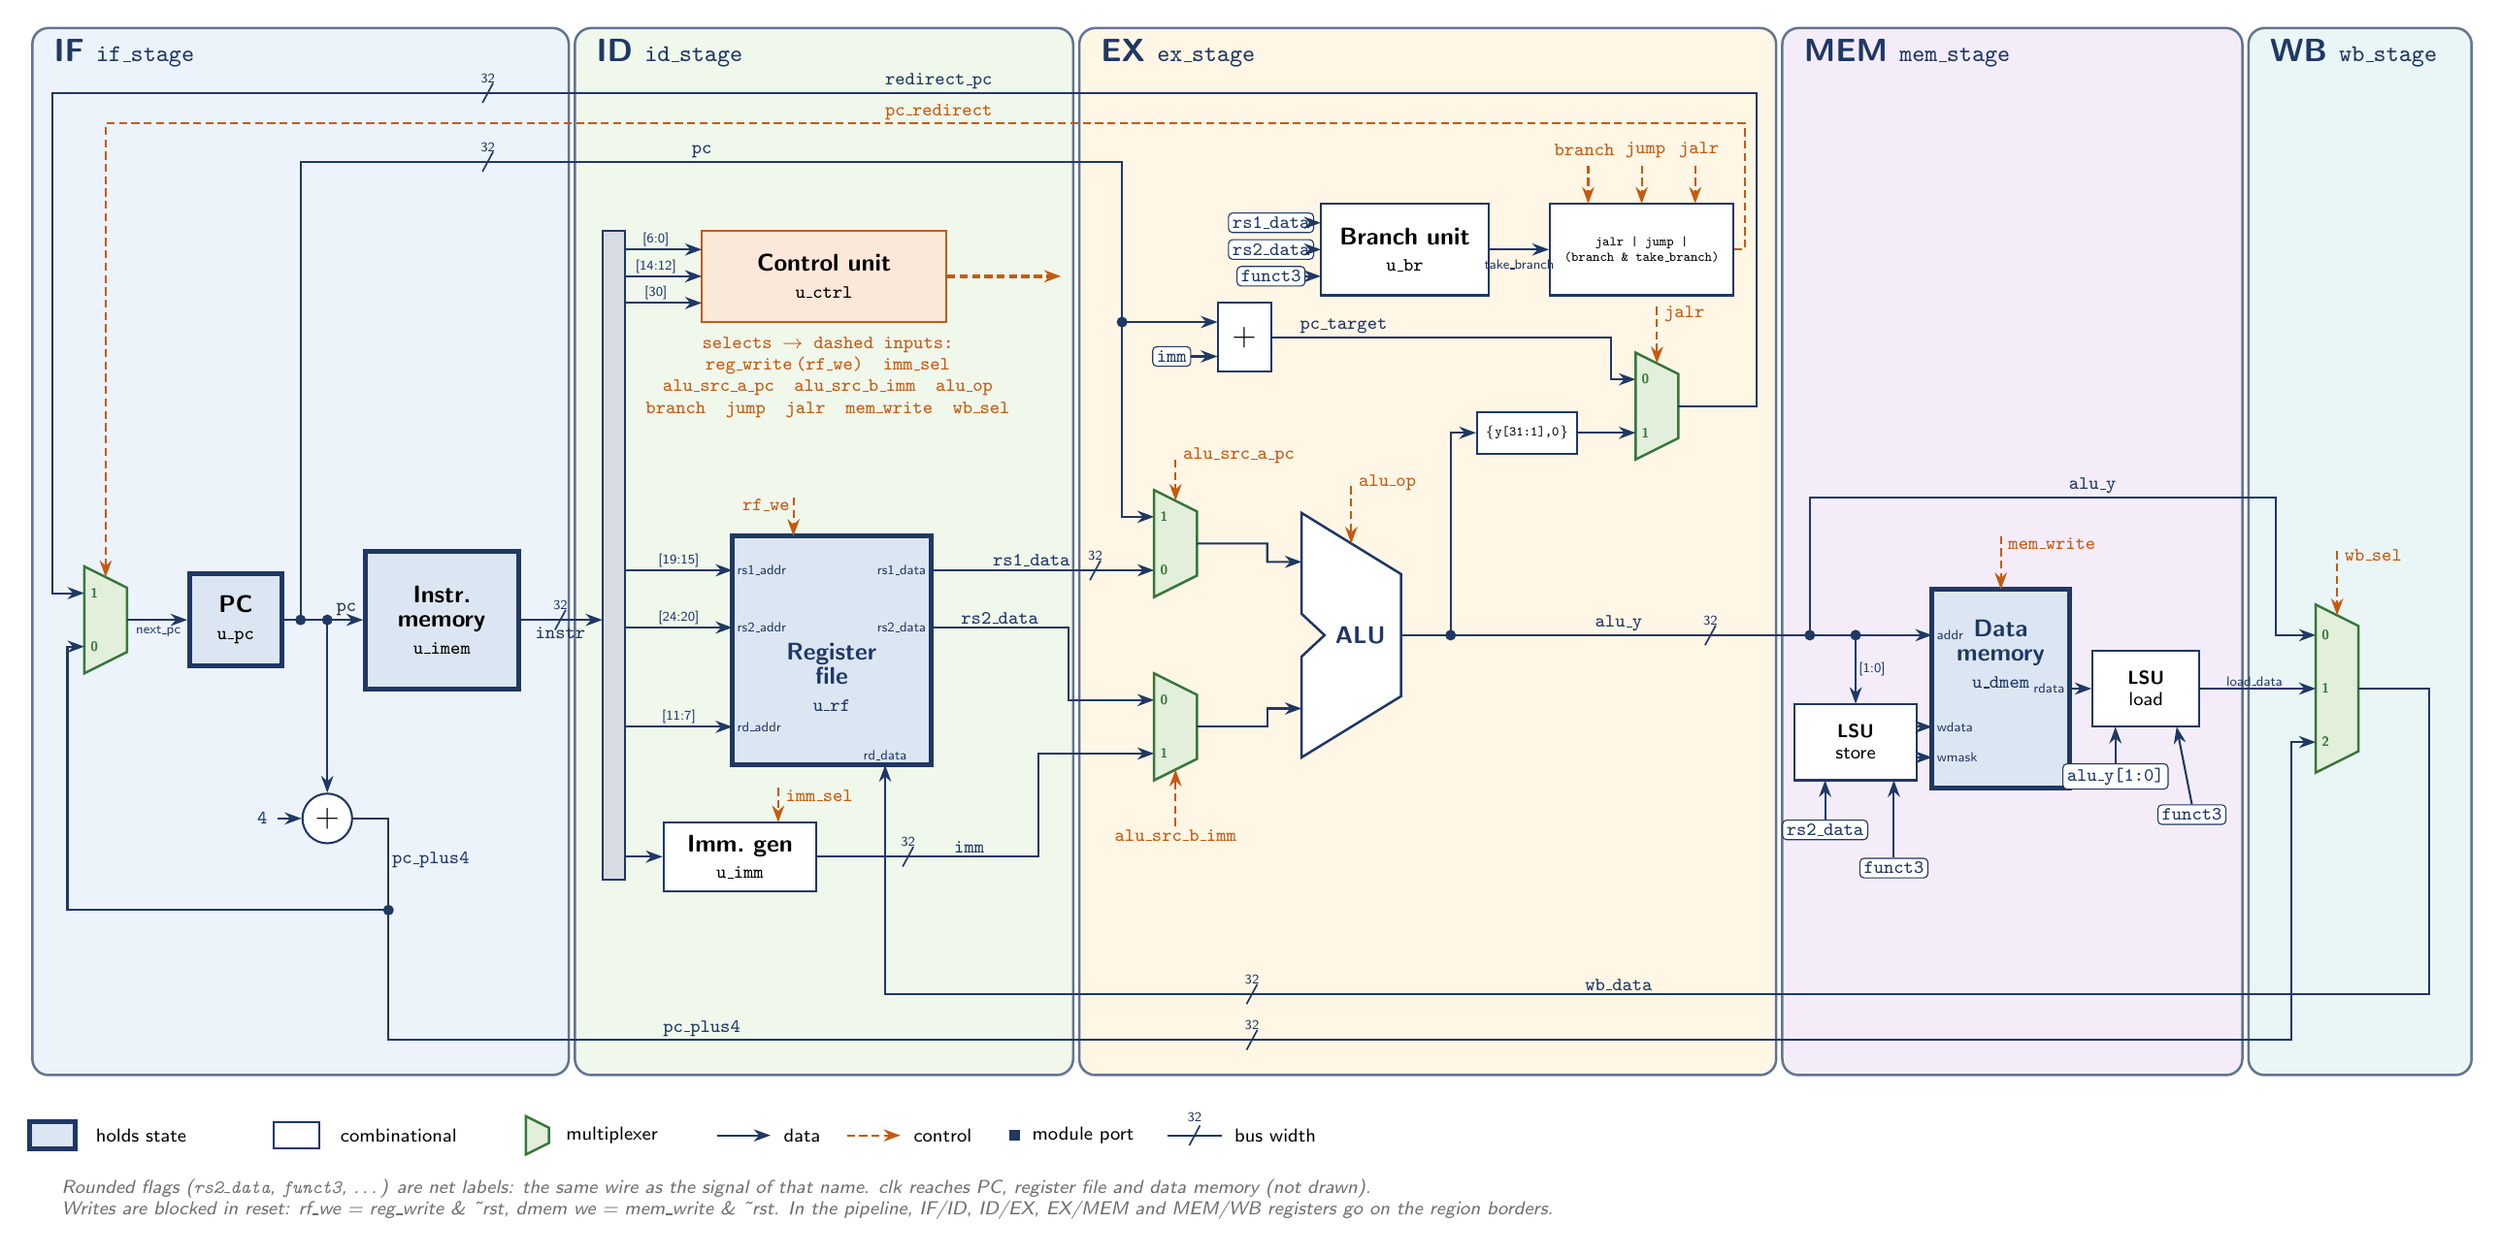
\begin{tikzpicture}
  % =================== stage regions ===================
  \foreach \x/\X/\c/\n/\m in {0/7.1/tintIF/IF/if\_stage, 7.1/13.7/tintID/ID/id\_stage,
                              13.7/22.9/tintEX/EX/ex\_stage, 22.9/29.0/tintMEM/MEM/mem\_stage,
                              29.0/32.0/tintWB/WB/wb\_stage} {
    \draw[stage, fill=\c] (\x+0.04,0.04) rectangle (\X-0.04,13.75);
    \node[title, anchor=west] at (\x+0.2,13.42) {\n\ \textmd{\small\ttfamily \m}};
  }

  % =================== IF ===================
  \muxR{npc}{1.0}{6.0}{1.4}
  \node[mlbl] at (0.85,6.35) {1};
  \node[mlbl] at (0.85,5.65) {0};
  \node[state, minimum width=12mm, minimum height=12mm] (pc) at (2.7,6.0) {\blk{PC}{u\_pc}};
  \node[state, minimum width=20mm, minimum height=18mm] (im) at (5.4,6.0) {\blkII{Instr.}{memory}{u\_imem}};
  \draw[data] (npc-out) -- (pc.west);
  \node[wlbl, below] at (1.69,5.95) {next\_pc};
  \draw[wire] (pc.east) -- (3.9,6.0);
  \node[dot] at (3.55,6.0) {};
  \node[dot] at (3.9,6.0) {};
  \draw[data] (3.9,6.0) -- (im.west);
  \node[sig, above] at (4.15,6.0) {pc};
  \node[addr] (a4) at (3.9,3.4) {+};
  \node[sig] at (3.05,3.4) {4};
  \draw[data] (3.25,3.4) -- (a4.west);
  \draw[data] (3.9,6.0) -- (a4.north);
  \draw[wire] (a4.east) -- (4.7,3.4) -- (4.7,2.2);
  \node[dot] at (4.7,2.2) {};
  \node[sig, right] at (4.7,2.85) {pc\_plus4};
  \draw[data] (4.7,2.2) -- (0.5,2.2) -- (0.5,5.65) -- (0.72,5.65);          % pc+4 -> next-PC mux
  \draw[data] (4.7,2.2) -- (4.7,0.5) -- (29.6,0.5) -- (29.6,4.4) -- (29.92,4.4);  % pc+4 -> WB mux
  \node[sig, above] at (8.8,0.5) {pc\_plus4};
  % pc forwarded to EX (over the top)
  \draw[data] (3.55,6.0) -- (3.55,12.0) -- (14.3,12.0) -- (14.3,7.35) -- (14.72,7.35);
  \node[sig, above] at (8.8,12.0) {pc};

  % =================== ID ===================
  \draw[data] (im.east) -- (7.5,6.0);
  \node[sig, below] at (6.95,5.95) {instr};
  \draw[draw=ink, fill=ink!18, line width=0.75pt] (7.5,2.6) rectangle (7.8,11.1);
  \node[ctrlblock, minimum width=32mm, minimum height=12mm] (cu) at (10.4,10.5) {\blk{Control unit}{u\_ctrl}};
  \draw[data] (7.8,10.85) -- node[wlbl, above, pos=0.4] {[6:0]}   (8.8,10.85);
  \draw[data] (7.8,10.5)  -- node[wlbl, above, pos=0.4] {[14:12]} (8.8,10.5);
  \draw[data] (7.8,10.15) -- node[wlbl, above, pos=0.4] {[30]}    (8.8,10.15);
  \draw[ctlnoarrow, line width=1.6pt, ->] (cu.east) -- (13.5,10.5);
  \node[csig, align=center, anchor=north] at (10.45,9.75)
       {selects $\rightarrow$ dashed inputs:\\reg\_write\,(rf\_we)\ \ imm\_sel\\alu\_src\_a\_pc\ \ alu\_src\_b\_imm\ \ alu\_op\\
        branch\ \ jump\ \ jalr\ \ mem\_write\ \ wb\_sel};
  \node[state, minimum width=26mm, minimum height=30mm] (rf) at (10.5,5.6) {};
  \node[align=center, font=\small, text=ink] at (10.5,5.25) {\blkII{Register}{file}{u\_rf}};
  \node[wlbl, anchor=west] at (9.23,6.65) {rs1\_addr};
  \node[wlbl, anchor=west] at (9.23,5.9)  {rs2\_addr};
  \node[wlbl, anchor=west] at (9.23,4.6)  {rd\_addr};
  \node[wlbl, anchor=south] at (11.2,4.13) {rd\_data};
  \node[wlbl, anchor=east] at (11.77,6.65) {rs1\_data};
  \node[wlbl, anchor=east] at (11.77,5.9)  {rs2\_data};
  \draw[data] (7.8,6.65) -- node[wlbl, above] {[19:15]} (9.2,6.65);
  \draw[data] (7.8,5.9)  -- node[wlbl, above] {[24:20]} (9.2,5.9);
  \draw[data] (7.8,4.6)  -- node[wlbl, above] {[11:7]}  (9.2,4.6);
  \draw[stub] (10.0,7.6) -- (10.0,7.1);
  \node[csig, anchor=east] at (10.0,7.5) {rf\_we};
  \node[block, minimum width=20mm, minimum height=9mm] (ig) at (9.3,2.9) {\blk{Imm.\ gen}{u\_imm}};
  \draw[data] (7.8,2.9) -- (ig.west);
  \draw[stub] (9.8,3.8) -- (9.8,3.35);
  \node[csig, anchor=west] at (9.85,3.7) {imm\_sel};
  % operands to EX
  \draw[data] (11.8,6.65) -- node[sig, above, pos=0.45] {rs1\_data} (14.72,6.65);
  \draw[data] (11.8,5.9) -- (13.6,5.9) -- (13.6,4.95) -- (14.72,4.95);
  \node[sig, above] at (12.7,5.9) {rs2\_data};
  \draw[data] (ig.east) -- (13.2,2.9) -- (13.2,4.25) -- (14.72,4.25);
  \node[sig, above] at (12.3,2.9) {imm};

  % =================== EX ===================
  \muxR{ma}{15.0}{7.0}{1.4}
  \node[mlbl] at (14.85,7.35) {1};
  \node[mlbl] at (14.85,6.65) {0};
  \draw[stub] (15.0,8.1) -- (ma-top);
  \node[csig, anchor=west] at (15.05,8.15) {alu\_src\_a\_pc};
  \muxR{mb}{15.0}{4.6}{1.4}
  \node[mlbl] at (14.85,4.95) {0};
  \node[mlbl] at (14.85,4.25) {1};
  \draw[stub] (15.0,3.3) -- (mb-bot);
  \node[csig, anchor=north] at (15.0,3.3) {alu\_src\_b\_imm};
  \aluR{alu}{17.3}{5.8}{3.2}
  \node[font=\bfseries\small, text=ink] at (alu-c) {ALU};
  \draw[stub] (17.3,7.75) -- (alu-op);
  \node[csig, anchor=west] at (17.35,7.8) {alu\_op};
  \draw[data] (ma-out) -- (16.2,7.0) -- (16.2,6.76) -- (alu-a);
  \draw[data] (mb-out) -- (16.2,4.6) -- (16.2,4.84) -- (alu-b);
  \draw[wire] (alu-out) -- (18.6,5.8);
  \node[dot] at (18.6,5.8) {};
  % pc + imm
  \node[block, minimum width=7mm, minimum height=9mm, font=\large] (add) at (15.9,9.7) {+};
  \node[dot] at (14.3,9.9) {};
  \draw[data] (14.3,9.9) -- (15.55,9.9);
  \node[flag] (fimm) at (14.95,9.45) {imm};
  \draw[data] (fimm.east) -- (15.55,9.45);
  \draw[data] (add.east) -- (20.7,9.7) -- (20.7,9.15) -- (21.02,9.15);
  \node[sig, above] at (17.2,9.7) {pc\_target};
  % jalr target and redirect mux
  \node[block, minimum width=13mm, minimum height=5.5mm, font=\tiny\ttfamily] (jt) at (19.6,8.45) {\{y[31:1],0\}};
  \draw[data] (18.6,5.8) -- (18.6,8.45) -- (jt.west);
  \muxR{rm}{21.3}{8.8}{1.4}
  \node[mlbl] at (21.15,9.15) {0};
  \node[mlbl] at (21.15,8.45) {1};
  \draw[data] (jt.east) -- (21.02,8.45);
  \draw[stub] (21.3,10.1) -- (rm-top);
  \node[csig, anchor=west] at (21.35,10.0) {jalr};
  % branch unit and redirect decision
  \node[block, minimum width=22mm, minimum height=12mm] (bu) at (18.0,10.85) {\blk{Branch unit}{u\_br}};
  \node[flag]  (f1) at (16.25,11.2)  {rs1\_data};
  \node[flag]  (f2) at (16.25,10.85) {rs2\_data};
  \node[flag]  (f3) at (16.25,10.5)  {funct3};
  \draw[data] (f1.east) -- (16.9,11.2);
  \draw[data] (f2.east) -- (16.9,10.85);
  \draw[data] (f3.east) -- (16.9,10.5);
  \node[block, minimum width=24mm, minimum height=12mm, font=\tiny\ttfamily] (rl) at (21.1,10.85)
        {jalr | jump |\\(branch \& take\_branch)};
  \draw[data] (bu.east) -- (rl.west);
  \node[wlbl, anchor=north] at (19.5,10.75) {take\_branch};
  \draw[stub] (20.4,11.95) -- (20.4,11.45);
  \draw[stub] (21.1,11.95) -- (21.1,11.45);
  \draw[stub] (21.8,11.95) -- (21.8,11.45);
  \node[csig] at (20.35,12.15) {branch};
  \node[csig] at (21.15,12.15) {jump};
  \node[csig] at (21.85,12.15) {jalr};
  % back to IF: pc_redirect (inner loop) and redirect_pc (outer loop)
  \draw[ctl] (rl.east) -- (22.45,10.85) -- (22.45,12.5) -- (1.0,12.5) -- (npc-top);
  \node[csig, above] at (11.9,12.5) {pc\_redirect};
  \draw[data] (rm-out) -- (22.6,8.8) -- (22.6,12.9) -- (0.3,12.9) -- (0.3,6.35) -- (0.72,6.35);
  \node[sig, above] at (11.9,12.9) {redirect\_pc};

  % =================== MEM ===================
  \draw[data] (18.6,5.8) -- (24.9,5.8);
  \node[sig, above] at (20.8,5.8) {alu\_y};
  \node[dot] at (23.3,5.8) {};
  \node[dot] at (23.9,5.8) {};
  \node[state, minimum width=18mm, minimum height=26mm] (dm) at (25.8,5.1) {};
  \node[align=center, font=\small, text=ink] at (25.8,5.55) {\blkII{Data}{memory}{u\_dmem}};
  \node[wlbl, anchor=west] at (24.93,5.8) {addr};
  \node[wlbl, anchor=west] at (24.93,4.6) {wdata};
  \node[wlbl, anchor=west] at (24.93,4.2) {wmask};
  \node[wlbl, anchor=east] at (26.67,5.1) {rdata};
  \draw[stub] (25.8,7.1) -- (25.8,6.4);
  \node[csig, anchor=west] at (25.85,7.0) {mem\_write};
  \node[block, minimum width=16mm, minimum height=10mm, font=\scriptsize] (ls) at (23.9,4.4) {\textbf{LSU}\\store};
  \draw[data] (23.9,5.8) -- node[wlbl, right] {[1:0]} (23.9,4.9);
  \draw[data] (24.7,4.6) -- (24.9,4.6);
  \draw[data] (24.7,4.2) -- (24.9,4.2);
  \node[flag]  (fs) at (23.5,3.25) {rs2\_data};
  \node[flag]  (ff) at (24.4,2.75) {funct3};
  \draw[data] (fs.north) -- (23.5,3.9);
  \draw[data] (ff.north) -- (24.4,3.9);
  \node[block, minimum width=14mm, minimum height=10mm, font=\scriptsize] (ll) at (27.7,5.1) {\textbf{LSU}\\load};
  \draw[data] (dm.east) -- (ll.west);
  \node[flag]  (fa) at (27.3,3.95) {alu\_y[1:0]};
  \node[flag]  (fg) at (28.3,3.45) {funct3};
  \draw[data] (fa.north) -- (27.3,4.6);
  \draw[data] (fg.north) -- (28.1,4.6);
  % alu_y on to WB
  \draw[data] (23.3,5.8) -- (23.3,7.6) -- (29.4,7.6) -- (29.4,5.8) -- (29.92,5.8);
  \node[sig, above] at (27.0,7.6) {alu\_y};

  % =================== WB ===================
  \muxR{wm}{30.2}{5.1}{2.2}
  \node[mlbl] at (30.05,5.8) {0};
  \node[mlbl] at (30.05,5.1) {1};
  \node[mlbl] at (30.05,4.4) {2};
  \draw[data] (ll.east) -- (29.92,5.1);
  \node[wlbl, above] at (29.12,5.1) {load\_data};
  \draw[stub] (30.2,6.9) -- (wm-top);
  \node[csig, anchor=west] at (30.25,6.85) {wb\_sel};
  \draw[data] (wm-out) -- (31.4,5.1) -- (31.4,1.1) -- (11.2,1.1) -- (11.2,4.1);
  \node[sig, above] at (20.8,1.1) {wb\_data};

  % =================== bus widths ===================
  \wmark{(6.95,6.0)}{32}
  \wmark{(13.95,6.65)}{32}
  \wmark{(11.5,2.9)}{32}
  \wmark{(22.0,5.8)}{32}
  \wmark{(6.0,12.0)}{32}
  \wmark{(6.0,12.9)}{32}
  \wmark{(16.0,1.1)}{32}
  \wmark{(16.0,0.5)}{32}

  % =================== legend and notes ===================
  \legend{0.3}{-0.75}
  \node[notetxt, anchor=north west] at (0.3,-1.2)
       {Rounded flags (\texttt{rs2\_data}, \texttt{funct3}, \dots) are net labels: the same wire as the signal of that name.
        clk reaches PC, register file and data memory (not drawn).\\
        Writes are blocked in reset: rf\_we = reg\_write \& \textasciitilde rst, dmem we = mem\_write \& \textasciitilde rst.
        In the pipeline, IF/ID, ID/EX, EX/MEM and MEM/WB registers go on the region borders.};
\end{tikzpicture}
\end{document}
